\documentclass[a4paper,twoside,11pt]{book}
%\documentclass[a4paper,twoside,11pt,titlepage]{book}
\usepackage{listings}
\usepackage[utf8]{inputenc}
\usepackage[spanish,es-tabla]{babel}
%%\usepackage{import} no lo encuentra, sirve para algo?
\usepackage[pdftex]{graphicx}
\usepackage{titlesec}
\usepackage{wrapfig}
\usepackage{url}
\usepackage{index}
\usepackage{enumitem}
\usepackage{caption}
\usepackage{booktabs} % Para formatos especiales de tablas
\usepackage{float}    % Posicionamiento avanzado de gráficos
\usepackage{subcaption} % Captions con figuras enlazadas
\usepackage{adjustbox}
\usepackage{amsmath}
\usepackage{amsfonts}
\usepackage{mathtools}

% Lista de acrónimos
\usepackage[acronym,shortcuts]{glossaries}
\makeglossaries
%
% Lista de acrónimos
% 
% Autor: Felipe Torres González
% Temática: WR-es
%
\newacronym{gnss}{GNSS}{Global Navigation Satellite System}
\newacronym{wr}{WR}{White-Rabbit}
\newacronym{ptp}{PTP}{Precision Time Protocol}
\newacronym{synce}{Sync-E}{Synchronous Ethernet}
\newacronym{ns}{ns}{nanosegundos}
\newacronym{hm}{H-maser}{Hydrogen maser}
\newacronym{ntp}{NTP}{Network Time Protocol}
\newacronym{gpsdo}{GPSDO}{GPS disciplined oscillator}
\newacronym{gps}{GPS}{Global Positioning System}
\newacronym{pps}{PPS}{Pulse Per Second}
\newacronym{lan}{LAN}{Local Area Network}
\newacronym{ieee}{IEEE}{Institute of Electrical and Electronics Engineers}
\newacronym{oc}{OC}{Ordinary Clock}
\newacronym{bc}{BC}{Boundary Clock}
\newacronym{gm}{GM}{GrandMaster}
\newacronym{tc}{TC}{Transparent Clock}
\newacronym{osi}{OSI}{Open System Interconnection}
\newacronym{bmc}{BMC}{Best Master Clock}
\newacronym{cern}{CERN}{Organización Europea para la Investigación Nuclear}
\newacronym{spec}{SPEC}{Simple PCIe FMC Carrier}
\newacronym{wrs}{WRS}{White Rabbit Switch}
\newacronym{soc}{SoC}{System on Chip}
\newacronym{fpga}{FPGA}{Field Programmable Gate Array}
\newacronym{wrc}{WRPC}{White Rabbit PTP Core}
\newacronym{wrc2p}{WRC2P}{White Rabbit Core Dual Port}
\newacronym{hdl}{HDL}{Hardware Description Language}
\newacronym{sma}{SMA}{SubMiniature version A}
\newacronym{ddmtd}{DDMTD}{Digital Dual Mixer Time Difference}
\newacronym{pll}{PLL}{Phase-locked loop}

%\usepackage{titlesec}
%\usepackage{pailatino}

\decimalpoint
\usepackage{dcolumn}
\newcolumntype{.}{D{.}{\esperiod}{-1}}
\makeatletter
\addto\shorthandsspanish{\let\esperiod\es@period@code}
\makeatother


%\usepackage[chapter]{algorithm}
\RequirePackage{verbatim}
%\RequirePackage[Glenn]{fncychap}
\usepackage{fancyhdr}
\usepackage{afterpage}

\usepackage{longtable}

\usepackage[pdfborder={000}]{hyperref} %referencia

% ********************************************************************
% Re-usable information
% ********************************************************************
\newcommand{\myTitle}{Arquitectura SoC-FPGA para aplicaciones de sincronzación de altas prestaciones}
\newcommand{\myDegree}{Máster en en Ciencia de Datos e Ingeniería de Computadores}
\newcommand{\myName}{Felipe Torres González}
\newcommand{\myProf}{Antonio Javier Díaz Alonso}
%\newcommand{\mySupervisor}{Put name here\xspace}
\newcommand{\myFaculty}{Escuela Técnica Superior de Ingenierías Informática y de
Telecomunicación\xspace}
\newcommand{\myFacultyShort}{E.T.S. de Ingenierías Informática y de
Telecomunicación\xspace}
\newcommand{\myDepartment}{Departamento de Arquitectura y Tecnología de Computadores}
\newcommand{\myUni}{\protect{Universidad de Granada}}
\newcommand{\myLocation}{Granada}
\newcommand{\myTime}{\today}
\newcommand{\myVersion}{Version 0.1}

% Algunos comandos más...
% Para inclinar el texto en las celdas de una tabla
\newcolumntype{R}[2]{%
    >{\adjustbox{angle=#1,lap=\width-(#2)}\bgroup}%
    l%
    <{\egroup}%
}
\newcommand*\rot{\multicolumn{1}{R{90}{1em}}}%
\renewcommand{\arraystretch}{1.2} % Aumentar el espacio entre filas de una tabla
\newcommand{\ra}[1]{\renewcommand{\arraystretch}{#1}}


\hypersetup{
pdfauthor = {\myName (felipetg<at>ugr.es},
pdftitle = {\myTitle},
pdfsubject = {},
pdfkeywords = {soc, fpga, white-rabbit, sincronización, ptp, timing}
pdfcreator = {latexmk},
pdfproducer = {pdflatex}
}

%\hyphenation{}


%\usepackage{doxygen/doxygen}
%\usepackage{pdfpages}
\usepackage{url}
\usepackage{colortbl,longtable}
\usepackage[stable]{footmisc}
%\usepackage{index}

\pagestyle{fancy}
\fancyhf{}
\fancyhead[LO]{\leftmark}
\fancyhead[RE]{\rightmark}
\fancyhead[RO,LE]{\textbf{\thepage}}
\renewcommand{\chaptermark}[1]{\markboth{\textbf{#1}}{}}
\renewcommand{\sectionmark}[1]{\markright{\textbf{\thesection. #1}}}

\setlength{\headheight}{1.5\headheight}

\newcommand{\HRule}{\rule{\linewidth}{0.5mm}}
%Definimos los tipos teorema, ejemplo y definición podremos usar estos tipos
%simplemente poniendo \begin{teorema} \end{teorema} ...
\newtheorem{teorema}{Teorema}[chapter]
\newtheorem{ejemplo}{Ejemplo}[chapter]
\newtheorem{definicion}{Definición}[chapter]

\definecolor{gray97}{gray}{.97}
\definecolor{gray75}{gray}{.75}
\definecolor{gray45}{gray}{.45}
\definecolor{gray30}{gray}{.94}
\definecolor{violet}{RGB}{0,0,153}

\lstset{ frame=Ltb,
     framerule=0.5pt,
     aboveskip=0.5cm,
     framextopmargin=3pt,
     framexbottommargin=3pt,
     framexleftmargin=0.1cm,
     framesep=0pt,
     rulesep=.4pt,
     backgroundcolor=\color{gray97},
     rulesepcolor=\color{black},
     %
     stringstyle=\ttfamily,
     showstringspaces = false,
     basicstyle=\scriptsize\ttfamily,
     commentstyle=\color{gray45},
     keywordstyle=\bfseries,
     %
     numbers=left,
     numbersep=6pt,
     numberstyle=\tiny,
     numberfirstline = false,
     breaklines=true
   }

% minimizar fragmentado de listados
\lstnewenvironment{listing}[1][]
   {\lstset{#1}\pagebreak[0]}{\pagebreak[0]}

\lstdefinestyle{CodigoC}
   {
	basicstyle=\scriptsize,
	frame=single,
	language=C,
	numbers=left
   }
\lstdefinestyle{CodigoC++}
   {
	basicstyle=\small,
	frame=single,
	backgroundcolor=\color{gray30},
	language=C++,
	numbers=left
   }

\lstdefinestyle{Consola}
   {basicstyle=\scriptsize\bf\ttfamily,
    backgroundcolor=\color{gray30},
    frame=single,
    numbers=none
   }


\newcommand{\bigrule}{\titlerule[0.5mm]}


%Para conseguir que en las páginas en blanco no ponga cabecerass
\makeatletter
\def\clearpage{%
  \ifvmode
    \ifnum \@dbltopnum =\m@ne
      \ifdim \pagetotal <\topskip
        \hbox{}
      \fi
    \fi
  \fi
  \newpage
  \thispagestyle{empty}
  \write\m@ne{}
  \vbox{}
  \penalty -\@Mi
}
\makeatother

\usepackage{pdfpages}

% Comentarios en línea a color
\newcommand{\incomment}[1]{\textcolor{violet}{\textit{#1}}}

% Cambio de los símbolos para las listas
\renewcommand{\labelitemi}{$\diamond$}
\renewcommand{\labelitemii}{$\bullet$}
\renewcommand{\labelitemiii}{$\circ$}
\renewcommand{\labelitemiv}{$\cdot$}

\begin{document}
\begin{titlepage}


\newlength{\centeroffset}
\setlength{\centeroffset}{-0.5\oddsidemargin}
\addtolength{\centeroffset}{0.5\evensidemargin}
\thispagestyle{empty}

\noindent\hspace*{\centeroffset}\begin{minipage}{\textwidth}

\centering

\includegraphics[width=0.9\textwidth]{imagenes/logo_ugr.png}\\[1.4cm]

\textsc{ \Large TRABAJO FIN DE MÁSTER\\[0.2cm]}
\textsc{
  MÁSTER DATCOM}\\[1cm]
% Upper part of the page
%
% Title
{\Huge\bfseries \myTitle}\\
% \noindent\rule[-1ex]{\textwidth}{3pt}\\[3.5ex]
%{\large\bfseries Subtitulo del Proyecto}
\end{minipage}

\vspace{2.5cm}
\noindent\hspace*{\centeroffset}\begin{minipage}{\textwidth}
\centering

\textbf{Autor}\\ {\myName} \\[2.5ex]
\textbf{Director} \\ {\myProf} \\[2cm]

\includegraphics[width=0.3\textwidth]{imagenes/etsiit_logo.png} \\[0.1cm]
\textsc{Escuela Técnica Superior de Ingenierías Informática y de Telecomunicación}\\
\textsc{---}\\
Granada, 8 de Septiembre, 2017
\end{minipage}
%\addtolength{\textwidth}{\centeroffset}
%\vspace{\stretch{2}}
\end{titlepage}

\chapter*{}
%\thispagestyle{empty}
%\cleardoublepage

%\thispagestyle{empty}

\begin{titlepage}


\setlength{\centeroffset}{-0.5\oddsidemargin}
\addtolength{\centeroffset}{0.5\evensidemargin}
\thispagestyle{empty}

\noindent\hspace*{\centeroffset}\begin{minipage}{\textwidth}

\centering
%
\includegraphics[width=0.9\textwidth]{imagenes/logo_ugr.jpg}\\[1.4cm]

%\textsc{ \Large PROYECTO FIN DE CARRERA\\[0.2cm]}
%\textsc{ INGENIERÍA EN INFORMÁTICA}\\[1cm]
% Upper part of the page
%

 \vspace{3.3cm}

%si el proyecto tiene logo poner aquí
%\includegraphics{imagenes/logo.png}
% \vspace{0.5cm}

% Title

{\Huge\bfseries \myTitle\\
}
\noindent\rule[-1ex]{\textwidth}{3pt}\\[3.5ex]
%{\large\bfseries Subtítulo del proyecto.\\[4cm]}
\end{minipage}

\vspace{2.5cm}
\noindent\hspace*{\centeroffset}\begin{minipage}{\textwidth}
\centering

\textbf{Autor}\\ {\myName}\\[2.5ex]
\textbf{Director}\\
{\myProf}\\[2cm]
%\includegraphics[width=0.15\textwidth]{imagenes/tstc.png}\\[0.1cm]
%\textsc{Departamento de Teoría de la Señal, Telemática y Comunicaciones}\\
%\textsc{---}\\
%Granada, mes de 201
\end{minipage}
%\addtolength{\textwidth}{\centeroffset}
\vspace{\stretch{2}}


\end{titlepage}




\cleardoublepage
\thispagestyle{empty}

\begin{center}
{\large\bfseries \myTitle}\\
\end{center}
\begin{center}
\myName\\
\end{center}

%\vspace{0.7cm}
\noindent{\textbf{Palabras clave}: White-Rabbit, Sincronización, PTP}\\

\vspace{0.7cm}
\noindent{\textbf{Resumen}}\\

Este proyecto trata sobre \incomment{terminar}
\incomment{importancia del timing, mencionar algo de wr y hablar de las 
aplicaciones}

\cleardoublepage


\thispagestyle{empty}


\begin{center}
{\large\bfseries SoC-FPGA architecture for high-accuracy synchronization 
applications}\\
\end{center}
\begin{center}
First name, Family name (student)\\
\end{center}

%\vspace{0.7cm}
\noindent{\textbf{Keywords}: Code optimization, assembly, PCGM, CUDA, SIMD, Fortran}\\

\vspace{0.7cm}
\noindent{\textbf{Abstract}}\\

This project is about the application of the acquired knowledge in many different degree`s subjects in order to optimize an algorithm of resolution of big systems of linear equations, named Preconditioned Conjugate Gradient Method (PCGM). It will apply many techniques of optimization in those areas where the compiler is not able to make the most of the own characteristics of the architecture objective of the build. In addition, it will try to utilise the implicit parallelism in the application that is implemented sequentially with the aim of using processors which profit efficiently the parallelism as the GPUs.

The used implementation is compared with another Fortran library very utilised in these areas, the NSPCG library, which does not profit completely the power of the calculation that is available. In order to improve the performance with respect to this library, it will be made several efforts. First, it will seek to optimize the CPU’s use by the employment of characteristics as the multimedia instructions that are able to make calculations in a vectorial way. Finally, through the utilization of another typical architecture of a computer as the GPU.

\chapter*{}
\thispagestyle{empty}

\noindent\rule[-1ex]{\textwidth}{2pt}\\[4.5ex]

Yo, \textbf{\myName}, alumno de la titulación \myDegree de la \textbf{Escuela 
Técnica Superior
de Ingenierías Informática y de Telecomunicación de la Universidad de Granada}, con DNI 15454650F, autorizo la
ubicación de la siguiente copia de mi Trabajo Fin de Máster en la biblioteca 
del centro para que pueda ser consultada por las personas que lo deseen.

\vspace{6cm}

\noindent Fdo: \myName

\vspace{2cm}

\begin{flushright}
Granada a 8 de Septiembre de 2017 .
\end{flushright}


\chapter*{}
\thispagestyle{empty}

\noindent\rule[-1ex]{\textwidth}{2pt}\\[4.5ex]

D. \textbf{\myProf}, Profesor del Departamento ATC de la Universidad de Granada.

\vspace{0.5cm}

\textbf{Informan:}

\vspace{0.5cm}

Que el presente trabajo, titulado \textit{\textbf{\myTitle}},
ha sido realizado bajo su supervisión por \textbf{\myName}, y autorizamos la 
defensa de dicho trabajo ante el tribunal que corresponda.

\vspace{0.5cm}

Y para que conste, expiden y firman el presente informe en Granada a X de Septiembre de 2017 .

\vspace{1cm}

\textbf{Los directores:}

\vspace{5cm}

\noindent \textbf{\myProf}

\chapter*{Agradecimientos}
\thispagestyle{empty}

       \vspace{1cm}


\incomment{aquí agradecimientos}

\frontmatter
\tableofcontents
\addcontentsline{toc}{chapter}{Índice de contenidos}
\listoffigures
\addcontentsline{toc}{chapter}{Índice de figuras}
\listoftables
\addcontentsline{toc}{chapter}{Índice de tablas}

\mainmatter
\setlength{\parskip}{5pt}

\chapter{Introducción}

El término sincronización hace referencia a la coordinación entre los múltiples 
elementos que componen un sistema para llevar a cabo alguna acción de forma 
simultánea en el tiempo. Mantener una noción común de tiempo es un factor clave 
en el que se basan muchas de las tecnologías que empleamos y de las que 
dependemos en nuestro día a día.

\incomment{El tiempo y la exactitud alcanzable como magnitud física.} Las 
fuentes más estables fabricadas hasta la fecha son los llamados relojes
atómicos. 
\incomment{Definir.} Estos son capaces de mantener un nivel de exactitud del 
orden de \gls{ns} por día, con una precisión igual a la frecuencia del
transmisor de radio que bombea el láser. \incomment{Explicar mejor y
referenciar.} \incomment{Encontrar ref a relojes ópticos de ROA}. Este tipo de 
soluciones alcanza valores de exactitud y precisión muy notables, sin embargo, 
su coste es muy elevado restringiendo el acceso a dichas fuentes de tiempo a la 
mayoría de laboratorios e instituciones que lo precisan. Los centros de 
metrología nacionales suelen ser los encargados de proveer la hora oficial del 
país en cuestión entre otros servicios ligados. Dichos centros cuentan con 
varias fuentes estables de tiempo como máseres de hidrógeno (suele
hacerse referencia al término por la contracción de su nombre en inglés: 
\acrshort{hm}) o relojes atómicos basados en patrones de haz de Cesio. 
Actualmente existe un gran interés por parte de estas entidades en el 
desarrollo de tecnologías que permitan realizar una distribución de sus 
referencias de tiempo de una manera estable y precisa.
Además de la distribución de tiempo, el campo del posicionamiento terrestre es 
otro de los grandes interesados en las tecnologías de sincronización. 
\incomment{Hablar de GNSS}. Para estos sistemas, \incomment{...}



\section{Motivación y Objetivos}

El gran interés mostrado tanto en el ámbito académico como en el industrial por 
mejorar los protocolos de sincronización actuales conlleva que cualquier 
trabajo en la línea de la sincronización tenga gran repercusión. En concreto la 
extensión del protocolo \gls{ptp} conocida como \gls{wr} está recibiendo mucha 
atención en los últimos años gracias al buen equilibrio entre prestaciones y 
coste de la tecnología así como a la existencia de diseños de referencia 
abiertos que fomentan el desarrollo de terceros.

La línea de este Trabajo Fin de Máster se encuadra en la dirección de la 
temática de mi futura tésis doctoral. Con la realización de este proyecto he 
podido asentar las bases de lo que será este futuro trabajo de investigación. 
Por un lado se ha detectado una posible vía de investigación en el ámbito de la 
sincronización basada en \gls{wr}, en concreto el estudio de como mejorar la 
arquitectura existente para lograr un sistema más eficiente, además de detectar 
cuales son los puntos críticos que están limitando la mejora tanto en exactitud 
como en precisión alcanzable por dicho protocolo. Por el otro, se ha podido 
asentar la base de conocimiento tanto en la propia tecnología de sincronización 
como en los aspectos relacionados: diseño basado en lógica reconfigurable, 
sistemas de recuperación de reloj, fuentes de ruido electromagnético, etc. que 
será de vital importancia para la consecución final de la citada tésis doctoral.

Por tanto, esta memoria refleja los primeros pasos necesarios para ello. En los 
capítulos 2 y 3 se introducen los conceptos teóricos clave para entender el 
trabajo. Se incluyen nociones clave para comprender el problema de la 
sincronización y las soluciones más relevantes que se han utilizado hasta la 
fecha. También se habla brevemente de temas de electrónica y de como se mide el 
ruido en estos sistemas \incomment{no me gusta}. En el capítulo 4 se habla de 
los componentes tecnológicos utilizados: tarjetas, entornos y herramientas de 
desarrollo, etc. El quinto capítulo contiene en análisis primigenio realizado 
para detectar puntos flacos y posibles cosas a mejorar en la arquitectura de un 
dispositivo \gls{wr}. El sexto capítulo trata la propuesta de la nueva 
arquitectura basada en \gls{soc} para nodos \gls{wr} y detalla algunas de las 
mejoras realizadas hasta la fecha. Los últimos capítulos contienen ideas para 
lo que será el trabajo futuro en esta línea y la conclusiones alcanzadas 
durante la realización de este trabajo.

Dado que este trabajo se engloba dentro de una línea más extensa que llevará 
varios años, se han planteado una serie de objetivos que tiene sentido alcanzar 
durante la realización de este trabajo y que se encuadran dentro de lo que será 
la posterior realización de la tesis doctoral:

\begin{itemize}
	\item Analizar el estado de la técnica de los principales protocolos 
	utilizados en sincronización de redes Ethernet, haciendo hincapié en el 
	nuevo protocolo denominado \gls{wr}.
	
	\item Analizar las limitaciones actuales de los nodos \gls{wr}.
	
	\item Proponer mejoras a la arquitectura de referencia de nodo.
	
	\item Analizar el sistema de recuperación de reloj y proponer mejoras para 
	conseguir aumentar las prestaciones en la sincronización 
\end{itemize}



\chapter{Mecanismos de sincronización en redes de computadores}

En este capítulo se detalla las características principales de los mecanismos 
empleados para la sincronización de equipos en red. Además se introducen los 
protocolos estándar más extendidos como \gls{ntp} o \gls{ptp} para llegar a una 
explicación más detallada sobre la extensión de \gls{ptp} conocida como 
\acrlong{wr}.

Los requisitos demandados por las aplicaciones que necesitan de algún mecanismo 
de sincronización son bastante heterogéneos. Esto es fácilmente entendible si 
se piensa en dos ejemplos de aplicaciones concretos: mantener la hora de 
sistema en los computadores de una red de propósito general, y hacerlo en los 
elementos de una fabrica de montaje de alta precisión.
En ambos escenarios se necesita de un mecanismo que permita mantener una misma 
noción de tiempo en los elementos del sistema, sin embargo en el primer 
escenario se puede tolerar un nivel de error que sería inaceptable en el 
segundo.
En otras aplicaciones, lo realmente importante es que todos los nodos de la red 
realicen una misma cuenta del tiempo, es decir, que la duración de un segundo 
sea lo más parecida en todos los nodos, sin importar tanto la fecha y la hora. 
En estos casos la sincronización se realiza mediante la distribución de una 
señal de reloj que se utiliza en los contadores internos de cada nodo. 

\section{Referencias de tiempo y frecuencia}

\section{Fuentes de ruido y desfase}

3.1.1 accuracy: The mean of the time or frequency error between the clock under 
test and a perfect
reference clock, over an ensemble of measurements. Stability is a measure of 
how the mean varies with
respect to variables such as time, temperature, and so on. The precision is a 
measure of the deviation of the
error from the mean.

\section{Network Time Protocol}

\textit{\acrlong{ntp}} \cite{Mills1991} es un protocolo estándar de red 
empleado para la sincronización de relojes en computadores conectados mediante 
redes conmutadas, que fue diseñado por David L. Mills de la Universidad de 
Delaware. Su uso se demostró públicamente por primera vez en 1979, en lo que 
sería una prueba de enlace satelital transatlántico para varios servicios de 
Internet. Posteriormente, en 1985 se implementó NTPv0 para sistemas tipo Unix 
donde la estructura para la cabecera y los cálculos para el tiempo de ida y 
vuelta (o \textit{round-trip time}) y el desfase entre relojes son los que se 
siguen utilizando en la versión actual NTPv4.

Los servidores \gls{ntp} pueden operar en varios modos: \textit{multicast}, 
llamada a procedimiento remoto y simétrico. El modo \textit{multicast} está 
enfocado a redes de área local (\gls{lan}) donde el número de clientes es 
grande y no se necesita de un alto nivel de precisión. En este escenario, uno o 
varios servidores se encuentran continuamente enviando mensajes de difusión 
\gls{ntp} que reciben los clientes que serán los encargados de calcular el 
desfase de su reloj con respecto al del servidor. Los servidores anuncian la 
posibilidad de proveer sincronización pero no aceptan mensajes \gls{ntp} de 
ninguno de los pares.
El segundo modo está pensado para escenarios donde se necesite una gran 
exactitud en la sincronización. Los servidores pueden actuar como cliente 
aceptando la sincronización de otro par (sin proveerla de forma descendente) o 
en modo servidor donde no aceptan ser sincronizados.
Los modos \textit{multicast} y llamada a procedimiento remoto no escalan bien 
en redes grandes de ámbito general como Internet. Para ello, los servidores de 
tiempo deben poder distribuirse de forma dinámica con una topología 
jerarquizada. Para este tipo de modo se emplea la comunicación simétrica donde 
el algoritmo de selección de \gls{ntp} determina el rol de cada uno de los 
servidores en la red.

\subsection{Organización de la red}

La topología de red usada en \gls{ntp} es de tipo jerárquica, donde el índice 
del nivel es un indicativo de la cercanía a la fuente primaria de tiempo. A 
cada nivel de la jerarquía se le denomina estrato. Se comienza a numerar por 0 
y se va sumando 1 por cada nivel de conexión en la jerarquía, es decir, un 
servidor sincronizado a un estrato \textit{n} se encontrará a \textit{n+1} 
saltos de la fuente principal. Este índice indica la distancia a la fuente y no 
necesariamente la calidad del servidor.

\begin{figure}
	\centering
	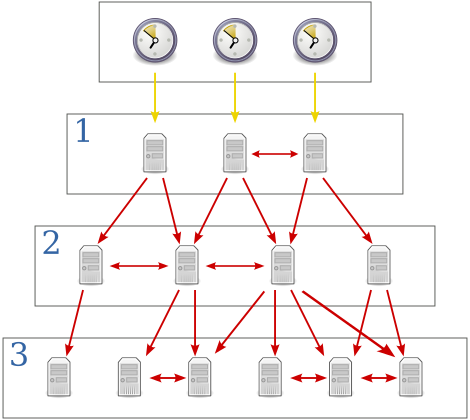
\includegraphics[width=0.7\linewidth]{imagenes/ntp_tree}
	\caption[Esquema de una red de distribución de tiempo usando NTP.]{En este 
	diagrama se 
	muestra una posible red de distribución de tiempo usando NTP. En el estrato 
	0 se hayan las fuentes de reloj de alta estabilidad como GPSDO o relojes 
	atómicos. Estas se conectan directamente a los servidores del estrato 1 que 
	forman los llamados servidores de tiempo primarios. Esta capa provee la 
	hora UTC al resto de los niveles. Como se puede ver se pueden establecer 
	enlaces entre equipos del mismo nivel, además, pueden estar conectados a 
	varios servidores de la capa superior (redundancia). Imagen tomada de 
	\cite{website:imgNTPtree}}
	\label{fig:ntptree}
\end{figure}


El límite superior para un estrato es el 15. Para indicar que un dispositivo no 
está sincronizado se utiliza el valor de estrato 16. El algoritmo \gls{ntp} 
está diseñado para construir una topología con los caminos más cortos hacía los 
servidores del estrato 1 (haciendo uso del algoritmo Bellman-Ford) lo que 
minimiza el tiempo de ida y vuelta acumulado entre los servidores de estrato 1 
y los clientes. A continuación se describen brevemente los estratos más 
relevantes:

\begin{itemize}
	\item \textbf{Estrato 0} \\ A este nivel se encuentran las fuentes de 
	tiempo de alta precisión, entre las que cabe destacar los relojes atómicos 
	o los osciladores disciplinados por GPS (\acrshort{gpsdo}). Generan una 
	señal de un pulso por segundo (\acrshort{pps}) que permite disciplinar el 
	oscilador interno del servidor conectado a la fuente de nivel 0.
	
	\item \textbf{Estrato 1} \\ Lo forman los servidores cuyos relojes se 
	disciplinan directamente con la señal recibida de una fuente de nivel 0 
	logrando una sincronización en torno a unos pocos microsegundos. Además 
	pueden conectarse con otros del mismo nivel para tareas de comprobación de 
	errores o para redundancia.
	
	\item \textbf{Estrato 2 (en adelante)} \\ Los dispositivos de cada estrato 
	se 
	sincronizan con el estrato anterior, pudiendo hacerlo con varios servidores 
	a la vez, y además pueden hacerlo con otros computadores del mismo nivel a 
	fin de mejorar la calidad del servicio.
\end{itemize}

\subsection{Algoritmo}

La figura \ref{fig:ntptree} muestra un esquema de organización típico para una 
red de distribución de tiempo usando \gls{ntp}. Para realizar el cálculo del 
desfase del reloj cliente con respecto al servidor, se emplean una serie de 
paquetes con marcas de tiempo (\textit{timestamps}). El cliente debe iniciar el 
proceso realizando una petición al servidor como muestra la figura 
\ref{fig:ntpts}. El servidor recibe el paquete y lo sella en el instante $T_i$. 
Para realizar los cálculos se emplean siempre las 4 marcas más recientes. Con 
ello se puede realizar el cálculo del tiempo de ida y vuelta ($\delta_i$), y el 
desfase del reloj ($theta_i$) del cliente con respecto al del sevidor en el 
instante de tiempo $T_i$:

\begin{equation}\label{ntprtt}
	\delta_i = (T_{i-2}-T_{i-3}) - (T_{i-1}-T_{i})
\end{equation}\label{ntpoffset}
\begin{equation}
	\theta_i = \frac{(T_{i-2}-T_{i-3}) + (T_{i-1}-T_{i})} {2}
\end{equation}

Hay que tener en cuenta que el servidor no tiene por qué contestar a las 
peticiones del cliente de forma inmediata. El proceso encargado de la gestión 
del servicio \gls{ntp} puede ser interrumpido por otra tarea con más prioridad, 
lo que hace que el tratamiento de las marcas de tiempo no sea determinista.

\begin{figure}
	\centering
	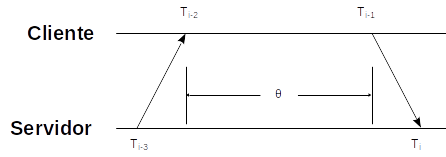
\includegraphics[width=0.7\linewidth]{imagenes/ntp_ts}
	\caption[Cálculo del desfase entre cliente y servidor]{La figura muestra un 
	intercambio de paquetes con marcas de tiempo entre cliente y servidor. Para 
	calcular el tiempo de ida y vuelta se utilizan 4 marcas de tiempo.}
	\label{fig:ntpts}
\end{figure}

\subsection{Rendimiento}

Al ser \gls{ntp} un protocolo que se implementa completamente en 
\textit{software}, no se consigue una gestión determinista para el cálculo del 
desfase entre las dos entidades que se sincronizan. Ello conlleva una 
limitación severa a la exactitud alcanzable mediante el uso de este protocolo 
\incomment{Mejorar esa frase}. Aunque este hecho podría ser tratado mediante el 
uso de sistemas operativos de tiempo real o técnicas que consigan reducir la 
latencia con la que el proceso encargado de la gestión del protocolo \gls{ntp} 
es ejecutado, existe otro factor de diseño que tiene incluso más peso en la 
precisión alcanzable por éste: la asunción de igualdad entre los caminos de ida 
y vuelta para los paquetes enviados por la red de comunicación. En \gls{ntp} se 
considera que el camino de transmisión de los paquetes es simétrico al camino 
de recepción, lo cual es bastante improbable en redes conmutadas con varios 
saltos y múltiples caminos como es el caso de Internet. Todo ello conlleva que 
la exactitud que alcanza este protocolo de forma general, sincronizando dos 
equipos, se sitúe en el orden de los milisegundos llegando a decenas de 
microsegundos en condiciones controladas.
\section{Precision time protocol}

Aunque el desarrollo del protocolo \gls{ntp} supuso un gran avance con respecto 
a las técnicas de sincronización en redes utilizadas anteriormente, la 
exactitud que podía alcanzar dicho protocolo no era suficiente para las 
aplicaciones con requisitos de altas prestaciones como los sistemas de control 
o sistemas de medición distribuidos. Para mejorar el rendimiento se propuso el 
desarrollo de un protocolo denominado \acrlong{ptp}, bajo el estándar 
\acrshort{ieee} 1588-2002 (año de su publicación) \cite{IEEE1588-2008}. 
Actualmente se utiliza la segunda revisión del estándar: IEEE 1588-2008 o 
\gls{ptp}v2, que no presenta compatibilidad con la versión anterior.

\subsection{Arquitectura de red}

El protocolo \gls{ptp} define una arquitectura jerárquica de tipo 
maestro-esclavo. Al igual que en la red \gls{ntp}, el nodo raíz puede estar 
conectado a una fuente estable de tiempo, como un \gls{gpsdo} o un reloj 
atómico, y provee de sincronización al resto de la red. En el caso de \gls{ptp} 
este nodo recibe el nombre de \acrlong{gm}. Los nodos intermedios pueden actuar 
como maestros del nivel siguiente o como nodos finales. A continuación se 
detallan las características más relevantes de los tipos de dispositivos más 
usuales:

\begin{itemize}	
	\item \textbf{\gls{oc}} \\
	Este tipo de nodos se comunican con el resto de la red via una única 
	intefaz de red física de tipo bidireccional que se encarga del intercambio 
	de los paquetes con las marcas de tiempo con el resto de la red. La 
	configuración de \gls{oc} sólo permite una única ejecución del 
	protocolo 
	\gls{ptp} y un único estado de funcionamiento. Así, este tipo de 
	configuración, permite al dispositivo actuar como maestro de la red 
	(\acrshort{gm}) o como reloj esclavo.
	
	\item \textbf{\gls{bc}} \\
	Los dispositivos que actúan como \acrshort{bc} suelen disponer de múltiples 
	puertos físicos que pueden actuar como si fuesen \gls{oc}s pero que 
	comparten una misma referencia de tiempo (recuperada del nodo maestro en el 
	nivel superior). Es decir, uno de los puertos se configurará como esclavo y 
	el resto podrán actuar como puertos maestros para los siguientes nodos de 
	la red.
	
	\item \textbf{\gls{tc}} \\
	La gran diferencia con respecto a los tipos anteriores reside en que los 
	\gls{tc} no se sincronizan con un nodo maestro. Estos actúan como simples 
	repetidores del tráfico entrante, pero modifican el campo de corrección de 
	los mensajes \textit{Follow\_UP o Pdelay\_Resp\_Follow\_UP} para incluir el 
	tiempo de residencia de los paquetes \gls{ptp} en el \gls{tc}. El campo de 
	corrección es usado posteriormente por los \gls{oc} para realizar el ajuste 
	de su reloj interno. 
	Dependiendo del mecanismo empleado para el cálculo del tiempo de 
	propagación se distinguen dos tipos de \gls{tc}: \textit{End-to-end} y 
	\textit{Peer-to-peer}.
\end{itemize}

\subsection{Algoritmo}

En el protocolo \gls{ptp} se distinguen dos fases de ejecución:
\begin{enumerate}
	\item Establecimiento de la jerarquía en la red.
	\item Sincronización de los relojes.
\end{enumerate}

En el arranque del algoritmo \gls{ptp} se espera por un lapso de tiempo a 
recibir mensajes de tipo \textit{Announce} provenientes de algún maestro en la 
red. Si no se reciben mensajes de ese tipo, el nodo asume que es maestro hasta 
que un maestro con mejores prestaciones aparezca en la red. La configuración de 
roles en la red se realiza mediante un algoritmo llamado \gls{bmc}, que utiliza 
varios parámetros como calidad de la fuente de reloj de un nodo o el nivel en 
el que se encuentra de la jerarquía (entre otras cosas) para decidir quien debe 
actuar como maestro en la red y quien como esclavo. Este ordenamiento se 
realiza de forma dinámica, de manera que si un nodo se cae, el resto de la red 
se vuelve a configurar en base a los nodos supervivientes.

Tras la fase de establecimiento de la jeraquía se pasa a la fase de 
sincronización, basada en el intercambio de una serie de paquetes 
con marcas de tiempo que permiten al nodo esclavo el cálculo del desfase de su 
reloj con respecto al de referencia en el nodo maestro. El proceso se describe 
en la Figura \ref{fig:ptpts}:

\begin{enumerate}
	\item El maestro manda un mensaje de tipo \textit{Sync} que es sellado 
	temporalmente en base a la escala del maestro en el momento de su envío. 
	Este mensaje puede contener su marca temporal ($T_1$) o necesitar de otro 
	tipo de 
	mensaje (\textit{Follow\_Up}) para transmitirla.
	
	\item El esclavo anota el tiempo de recepción (en su propia escala de 
	tiempo) del mensaje en la marca $T_2$.
	
	\item El esclavo manda un mensaje de tipo \textit{Delay\_Req} al maestro y 
	almacena la marca de tiempo en que lo hace ($T_3$).
	
	\item El maestro sella la recepción del paquete recibido y la envía dentro 
	de un paquete de tipo \textit{Delay\_Resp} ($T_4$).
\end{enumerate}

Una vez el esclavo dispone de las cuatro marcas de tiempo, se procede al 
cálculo del tiempo de propagación en una dirección y del desfase entre relojes 
para poder corregir el reloj en el nodo esclavo.

\begin{equation}\label{delmm}
delay_{mm} = (T_4 - T_1) - (T_3 - T_2)
\end{equation}

\begin{equation}\label{delms}
	delay_{ms} = \frac {1} {2} delay_{ms}
\end{equation}

\begin{equation}\label{offset}
	offset = T_2 - T_1 - delay_{ms}
\end{equation}

Como en el caso de \gls{ntp}, se considera que el tiempo de propagación de los 
mensajes en el camino de ida es igual al de vuelta. En un escenario realista 
esto no tiene por qué cumplirse. Por tanto, cualquier asimetría existente 
introduce un error en el cómputo del valor de desfase.

Los mensajes \gls{ptp} se pueden clasificar dentro de dos clases: mensajes de 
evento y mensajes generales. Todos los mensajes de tipo evento son sellados 
temporalmente tanto en el momento de la emisión como en el de la recepción. 
Dicha marca temporal indica el momento en el que un paquete abandona un nodo y 
entra en el medio de transmisión y viceversa. Con ello se obtienen las 4 
marcas de tiempo necesarias en el cálculo del tiempo de propagación y del 
desfase entre relojes.

Los mensajes de tipo evento son los siguientes:


\begin{itemize}
	
	\item \textbf{Sync} \\
	Es un mensaje transmitido de maestro a esclavo que permite medir el retardo 
	de propagación para un paquete en dicho sentido de la comunicación. Para 
	ello 
	se sella temporalmente el paquete al ser enviado por el maestro y se 
	acompaña dicha marca de tiempo al paquete (o se envía en otro paquete 
	posterior de tipo \textit{Follow\_Up}) para que el nodo esclavo pueda 
	realizar los cálculos. Estos paquetes proporcionan las marcas temporales 
	$T_1 y T_2$.
	
	\item \textbf{Delay\_Req} \\
	Este mensaje lo sella temporalmente el nodo esclavo y lo envía al maestro 
	para obtener la marca temporal de recepción en otro paquete de respuesta 
	denominado \textit{Delay\_Resp}, obteniendo así las marcas $T_3$ y $T_4$, 
	que 
	junto a las dos anteriores permiten calcular el tiempo de ida y vuelta, y a 
	partir de este el desfase de los relojes.
\end{itemize}

En \gls{ptp} se puede medir el retraso producido por la transmisión de los 
paquetes en la red de dos formas distintas. En una modalidad el intercambio de 
paquetes se realiza como muestra la Figura \ref{fig:ptpts}. En ella el cálculo 
del desfase se realiza siempre entre pares de 
dispositivos \gls{ptp} conectados sin tener en cuenta al resto. Esto se 
denomina \textit{end-to-end}.
La otra modalidad consiste en considerar los nodos intermedios entre el nodo 
maestro de la red y el esclavo de turno como si fueran un cable. Para ello, 
los nodos intermedios deben añadir el retardo que supone que los paquetes 
los atraviesen, en un campo del paquete denominado \textit{Correction 
Field}. El esclavo se sincronizará en relación a las marcas de tiempo del 
maestro principal y le sumará los retardos mencionados. A este método se le 
llama \textit{peer-to-peer}.

\textit{Peer-to-peer} tiene la ventaja de no añadir complejidad en el sistema 
ocasionado por varios niveles de dispositivos sincronizándose (encadenar bucles 
de control suele elevar los niveles de ruido del sistema) pero necesita que los 
dispositivos intermedios sean compatibles y sepan modificar el campo 
\textit{correction field}. En caso contrario el nivel de error en la 
sincronización será elevado. El caso de \textit{end-to-end} es más flexible en 
ese aspecto ya que mide el tiempo de ida y de vuelta con el maestro local 
permitiendo corregir mejor los efectos de atravesar dispositivos no compatibles.

Además de los tipos de mensajes listados anteriormente, existen mensajes 
especiales para el modo \textit{peer-to-peer}. Dado que actualmente el protoclo 
\gls{wr} solo implementa comunicación \textit{end-to-end} se omite la 
explicación de los mismos, que puede ser consultada en \cite{IEEE1588-2008}. En 
la actualidad se está desarrollando el soporte para \textit{peer-to-peer} y 
\gls{tc}, para más información se puede consultar \incomment{preguntar a JL}.

\begin{figure}
	\centering
	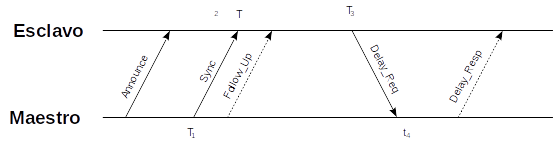
\includegraphics[width=0.7\linewidth]{imagenes/ptp_ts}
	\caption[Intercambio de mensajes para el algoritmo de \acrshort{ptp}]{La 
	figura muestra la secuencia de intercambio de mensajes 
	que se emplea en el algoritmo de \gls{ptp} para conseguir las 4 marcas de 
	tiempo necesarias en el cálculo del \textit{round-trip time} y del desfase.}
	\label{fig:ptpts}
\end{figure}

Para la clase de mensajes generales caben ser destacados los siguientes:

\begin{itemize}
	\item \textbf{Announce} \\
	Es el tipo de mensaje utilizado para informar al resto de los nodos acerca 
	del nodo que transmite (estado y características) además de quién es su 
	\gls{gm}. Son utilizados por el algoritmo \gls{bmc}.
	
	\item \textbf{Follow\_Up} \\
	Sirve para transmitir la marca de tiempo en la escala del maestro para la 
	emisión del mensaje \textit{Sync}.
	
	\item \textbf{Delay\_Resp} \\
	Análogo al anterior para el caso del mensaje \textit{Delay\_Req}.
	
	\item \textbf{Gestión y señalización} \\
	Se engloban mensajes para control y gestión de los relojes o para 
	transmitir información general de estado entre los nodos.
	
\end{itemize}


\subsection{Rendimiento}

Como se ha visto la esencia del mecanismo de sincronización de \gls{ptp} es 
similar al visto anteriormente en la sección de \gls{ntp}: se intercambian una 
serie de paquetes con marcas de tiempo entre dos nodos de la red para calcular 
el desfase entre sus relojes, entonces ¿cómo se consigue la mejora? La gran 
diferencia entre ambos protocolos es la inclusión en el primero del sellado de 
tiempo a nivel de \textit{hardware}. Cuando un paquete de tipo \gls{ptp} llega 
a un puerto, este genera un evento para que una lógica especial realice un 
sellado de tiempo de dicho paquete. Dicha lógica se encuentra entre la capa 
física (PHY) y la capa de enlace (MAC) del modelo \acrshort{osi} 
(\textit{\acrlong{osi}}). Este mecanismo evita la latencia que supone el 
procesamiento de los paquetes y el sellado de tiempo a nivel de 
\textit{software}. Otra diferencia significativa entre \gls{ntp} y \gls{ptp} se 
encuentra en la gestión de las colas de recepción/envío que son fuente de 
retardos no deterministas. Gracias al sellado con soporte \textit{hardware} y 
al tratamiento de los retardos ocasionados por las colas, \gls{ptp} consigue 
una precisión de decenas de nanosegundos con las técnicas más avanzadas 
actualmente. \incomment{referenciar algo}




\section{White Rabbit}

\acrfull{wr} hace referencia tanto al protocolo diseñado como mejora de 
\gls{ptp}v2 como al proyecto internacional que se encarga de su desarrollo y 
mantenimiento. Inicialmente parte como una tecnología desarrollada por el 
\gls{cern} para actualizar el sistema de sincronización y envío de datos de 
control para su complejo de aceleradores de partículas. Gracias a el espíritu 
abierto con el que se desarrolló la tecnología (y a su prometedor rendimiento) 
fueron sumándose otras instituciones al desarrollo, tanto desde el ámbito 
académico, donde cabe destacar el Centro de Investigación de Iones Pesados 
(\textit{Gesellschaft für Schwerionenforschung}, GSI en alemán) en Alemania o 
la propia Universidad de Granada; como desde el empresarial, donde se está 
intentando expandir la tecnología al ámbito industrial. Ejemplos de ello son la 
empresa Seven Solutions (\text{spin-off} de la UGR) en Granada, o CreoTECH en 
Polonia. 

Aunque el empuje en el ámbito de la ciencia es mucho más 
evidente gracias a la inclusión de \textit{WR} en instalaciones para 
aceleradores de partículas, institutos metrológicos o en sistemas de 
adquisición ditribuida como el caso del proyecto Square Kilometre Array (SKA) 
que se está contruyendo en Sudáfrica y que una vez concluido será el 
instrumento de observación astronómica más sensible jamás construido por la 
humanidad. En el caso de la empresa privada, \gls{wr} se ve todavía como una 
tecnología muy prometedora para diversas áreas como Smart Grid, 
Geo-posicionamiento o para las telecomunicaciones, que aún necesita madurar. 
Esto está a punto de cambiar gracias a su inclusión en la próxima revisión del 
estándar \gls{ptp} bajo un nuevo perfil de alta precisión.

Los objetivos de desarrollo iniciales estaban enfocados al entorno de los 
aceleradores de partículas, priorizando una sincronización de calidad junto a 
un sistema que fuese determinista y fácil de mantener:

\begin{itemize}
	\item Lograr para una red de miles de nodos, conectados por enlaces de 
	fibra óptica de hasta 10 km, una diferencia menor del nanosegundo entre dos 
	nodos cualesquiera de la red, es decir, una exactitud de sincronización 
	\textbf{sub-nanosegundo}. Además, se requiere una precisión en el orden del 
	picosegundo.
	
	\item Permitir que el enlace utilizado para los paquetes del protocolo 
	\gls{wr} se pueda \textbf{compartir para} el envío de \textbf{datos de 
	propósito general}, 
	reduciéndo así costes en el despliegue de las infraestructuras.
	
	\item Realizar un desarrollo \textbf{simple y escalable} que no necesite de 
	sofisticados procedimientos de configuración o calibración.
	
	\item Establecer un envío \textbf{determinista} para los paquetes 
	prioritarios, con 
	retardos que no superen ciertos valores umbrales. Esto es especialmente 
	importante en sistemas de control donde la respuesta a un evento no puede 
	exceder un tiempo límite en su envío.
	
	\item Proveer un \textbf{diseño} de referencia \textbf{abierto} a la 
	comunidad 
	(tanto \textit{hardware} como \textit{software}) para fomentar el 
	desarrollo por parte de esta, y evitar las ligaduras con fabricantes.
\end{itemize}

En la actualidad se puede afirmar que en su mayor parte se han cumplido dichos 
objetivos. El requisito principal de rendimiento es algo que se ha conseguido 
en su mayor parte aunque hace falta aportar datos acerca del comportamiento del 
protocolo en redes realmente grandes con un gran número de nodos. La tendencia 
actual en cuanto a rendimiento se centra en la mejora de la exactitud alcanzada 
en escenarios no tan típicos, como enlaces de larga distancia o escenarios con 
cambios en las condiciones de operación. También se investiga como reducir el 
ruido producido por los componentes del sistema de sincronización para lograr 
una precisión en el orden del femtosegundo. El envío determinista es algo que 
no siempre se logra, ya que se puede producir la pérdida de algún paquete de 
alta prioridad en casos de congestión del enlace. Las herramientas de gestión y 
mantenimiento es otro punto al que todavía le queda trabajo por delante y al 
que se está prestando bastante atención dado que son algo crucial si se 
pretende extender el uso del protocolo más allá del ámbito científico.

El protocolo \gls{wr} fue diseñado como una extensión del protocolo IEEE 
1588-2008 (\gls{ptp}v2) al que se añadieron varias mejoras como un modelo de 
enlace más preciso, técnicas de calibración automática o sintonización de los 
relojes mediante el envío de la frecuencia maestra codificada en los paquetes 
transmitidos.




\chapter{Análisis limitaciones actuales} \label{cap:cadena}

El proyecto \gls{wr} ofrece dos tipos de arquitectura como referencia: la 
orientada a dispositivos que actúen como \gls{bc}, y la enfocada a nodos 
finales \gls{oc}. En la sección \ref{sec:wr} se ha visto que para la primera se 
cuenta con un dispositivo de referencia, el \gls{wrs}, que implementa la 
arquitectura 
de \gls{bc} y en la cual se centra el desarrollo del \textit{OHWR}. La segunda 
se materializa en la tarjeta \gls{spec} como ejemplo básico de nodo \gls{wr}.

La línea de desarrollo seguida desde la empresa Seven Solutions y desde el 
grupo de investigación enfocado en \gls{wr} de la UGR se ha centrado en el 
desarrollo de las arquitecturas de referencia y en el diseño de nuevos tipos de 
arquitecturas que solucionen las deficiencias presentes en los diseños 
iniciales.

Aunque la estrategía no es la misma si se habla de la arquitectura de 
\textit{switch} que si se hace de la de nodo, si es cierto que hay una 
corriente que se comparte en ambos desarrollos: la utilización de los nuevos 
modelos de \gls{soc} para lograr un mayor nivel de integración y un aumento de 
las prestaciones del sistema sin elevar la complejidad del mismo en exceso.

En el caso del \gls{wrs} existente se han detectado varios problemas por la 
gran complejidad del diseño \textit{hardware} que tiene el circuito 
electrónico. 
Uno de ellos es la comunicación entre el procesador ARM y el circuito  
implementado en la lógica reconfigurable de la \gls{fpga}. Gracias a la mejora 
en la 
tecnología de fabricación se consiguen actualmente sistemas que integran tanto 
\gls{fpga} como microprocesador en un único chip reduciendo costes y 
complejidad de desarrollo.

La arquitectura referencia para los nodos \gls{wr} ha tratado de ofrecer un 
diseño básico y asequible económicamente. El uso de la familia Spartan de 
Xilinx ha permitido mantener los costes bajos a la vez que ha permitido alojar 
el diseño básico de la arquitectura de nodo \gls{wr} . Sin embargo, dicho 
diseño se está mejorando y está recibiendo cada vez más funcionalidades por lo 
que la necesidad de recursos está creciendo. Además, dicho diseño tiene una 
limitación bastante importante: carece de un microprocesador dedicado lo que 
dificulta en gran medida el desarrollo e incorporación de nuevas 
características. De igual forma que en la arquitectura de \textit{wrs} se 
tiende hacía soluciones en \gls{soc}, la arquitectura de nodo se puede 
beneficiar de este tipo de soluciones ya que permiten incluir un 
microprocesador físico en el diseño sin necesidad de gastar puertas para 
incluirlo y además mantener los costes bajos.

Mi trabajo de investigación se ha enfocado en la arquitectura de nodo por lo 
que será a la que haga referencia en el resto de la memoria, aunque como he 
comentado en los párrafos anteriores, muchas de las mejoras planteadas a 
continuación se pueden incorporar en la arquitectura tipo \textit{switch}.

El primer paso para poder plantear mejoras a la arquitectura de nodo y al 
rendimiento de la sincronización en los mismos es establecer el punto de 
partida. Para ello se ha realizado una labor de análisis de una arquitectura 
actual de nodo basada en un diseño similar al de la tarjeta SPEC pero 
que ya presenta una serie de mejoras.

El nodo utilizado como punto de partida es el WR-LEN \cite{website:len}. Dicho 
dispositivo incorpora una versión 
mejorada del \gls{wrc} denominado \gls{wrc2p} cuya principal característica es 
la inclusión de un segundo puerto físico a la arquitectura de nodo.

\subsection{White Rabbit Core Dual Port}

El \gls{wrc2p} \cite{felipe16} es una extensión de la arquitectura para nodos 
\gls{wr} 
denominada \acrlong{wrc} \cite{Daniluk2012} que añade una segunda interfaz 
física 
Ethernet a la arquitectura básica mono-puerto. En la implementación actual, la 
referencia temporal es única para ambos puertos, lo que supone que el 
dispositivo puede actuar como nodo (esclavo o maestro) y como \gls{bc}, es 
decir, esclavo de un nivel superior de la jerarquía de red y maestro de un 
nivel inferior. Además, se pretenden desarrollar técnicas que habiliten la 
redundancia (hacer un cambio de referencia si un enlace se cae).

Esta nueva arquitectura de nodo extendida permite el desarrollo de dispositivos 
\gls{bc} de coste reducido que son ideales para su uso en topologías lineales, 
donde el uso de \gls{wrs}s supone una infrautilización de los puertos 
disponibles por equipo.

\begin{figure}
	\centering
	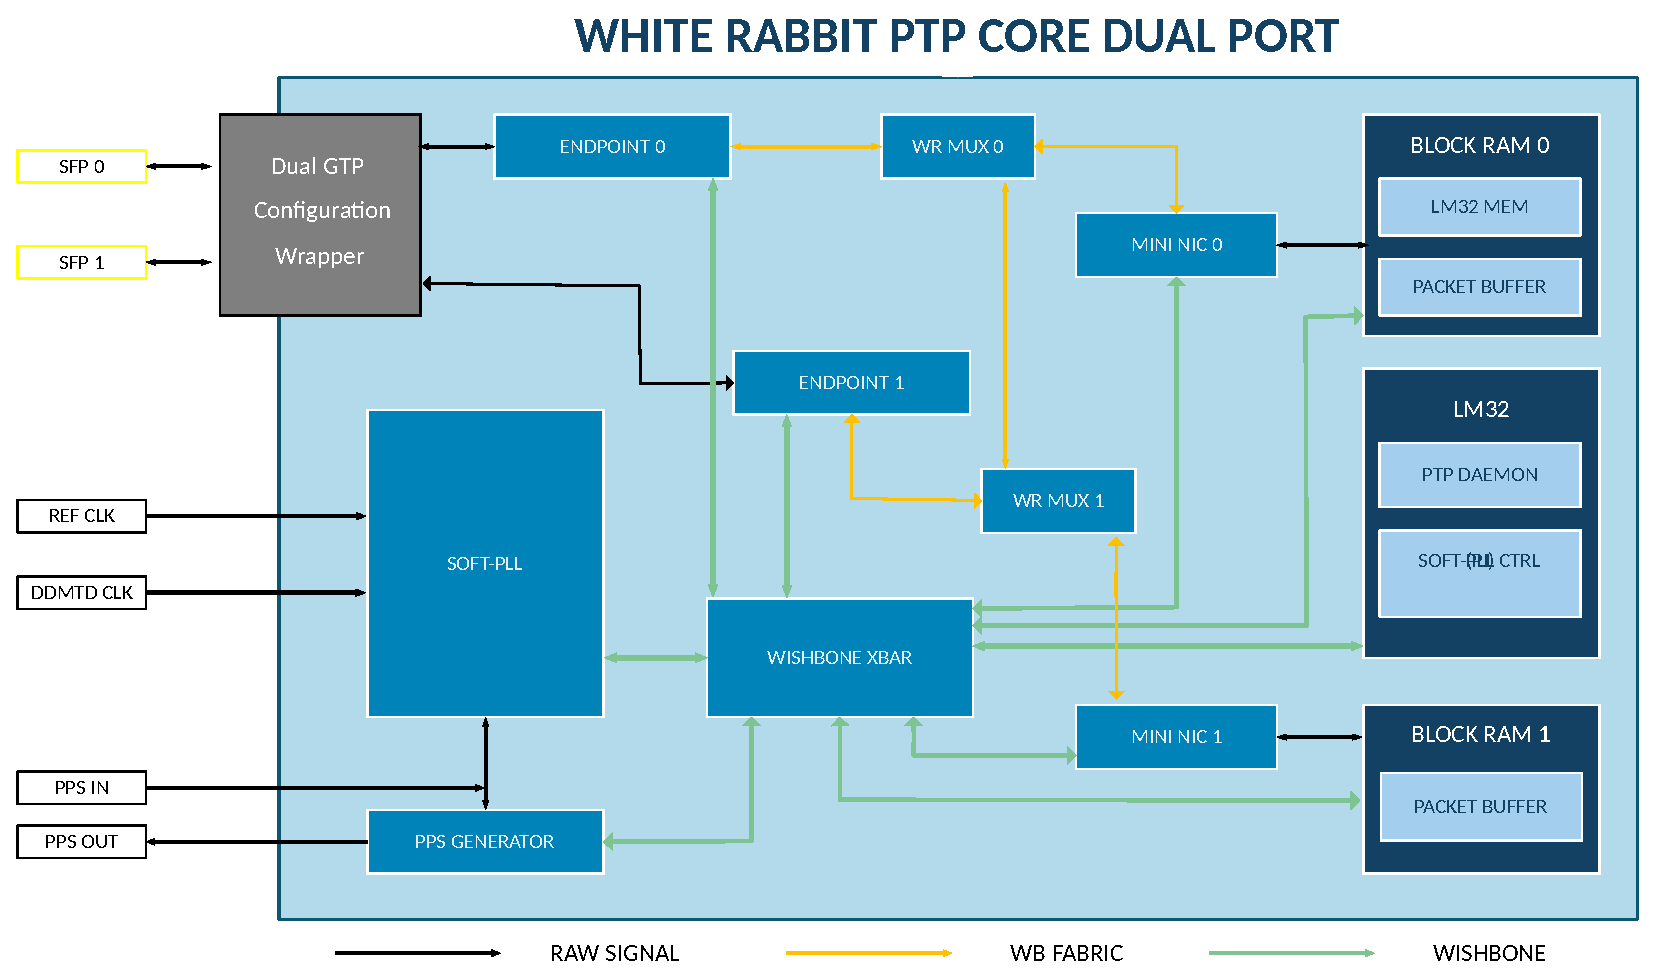
\includegraphics[width=\linewidth]{imagenes/wrpc_dp}
	\caption[Diagrama de bloques del WRC2P]{Este diagrama muestra la estructura 
	de módulos HDL para el diseño de la arquitectura WRC2P.}
	\label{fig:wrpcdp}
\end{figure}


La Figura \ref{fig:wrpcdp} muestra como se organizan los módulos para la 
arquitectura de \gls{fpga}. Con respecto al diseño de referencia se realiza una 
duplicación de los componentes principales de la lógica de \gls{wr}: 
\textit{endpoint}, multiplexor WR, mini-NIC
y los módulos de RAM. Sin embargo el bloque para el procesador embebido se 
mantiene, realizando únicamente cambios a nivel de \textit{sw}. Con ello se 
consigue reducir el número de puertas necesarias, algo clave para alojar la 
arquitectura dentro de una FPGA de perfil bajo.

\subsection{WR-LEN}

El WR-LEN es el primer dispositivo \gls{wr} en incorporar la arquitectura 
\gls{wrc2p}. Sus principales características son la inclusión de un segundo 
puerto físico compatible con \gls{wr}, conectores coaxiales de tipo \gls{sma} y 
una tercera interfaz Ethernet de tipo 1000BaseT.

\begin{figure}
	\centering
	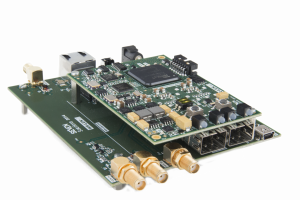
\includegraphics[width=0.7\linewidth]{imagenes/wrlen}
	\caption[WR-LEN en su versión para desarrolladores]{Imagen de un equipo 
	WR-LEN sin caja. Se puede observar como se compone de dos tarjetas: la 
	principal (arriba) donde se sitúa la electrónica de control de WR, y el 
	\textit{backplane} (abajo) que dota de interfaces de entrada/salida a la 
	primera.}
	\label{fig:wrlen}
\end{figure}


La electrónica encargada de la recuperación de reloj y mantenimiento de la 
referencia de tiempo local se mantiene con respecto a la utilizada en el 
\gls{wrs}. El oscilador principal es un modelo que compensa el cambio de 
temperatura y permite el ajuste de la frecuencia por medio de voltaje (VCTCXO) 
Mercury VM53S3. También se ha mantenido el \gls{pll} que se encarga de generar 
las frecuencias necesarias para la lógica de control de WR es el AD9516-4 de 
Analog Devices. Un cambio reseñable se encuentra en el reloj utilizado 
para los módulos 
\gls{ddmtd} que ya no utiliza un \gls{pll} externo para generar la frecuencia 
de 62.5 MHz necesaria, si no que se aprovecha uno de los \gls{pll} internos de 
la \gls{fpga} para ello.

\subsection{Experimentos de escalabilidad}

Para evaluar las limitaciones del \gls{wrc2p} en cuanto a prestaciones y 
escalabilidad realicé una serie de experimentos encadenando múltiples nodos 
\gls{wr} \cite{felipe16}. A través del análisis de la señal de reloj de salida 
producida por 
la lógica de \gls{wr} se pueden obtener indicadores de como de estable es el 
proceso de sincronización en cada nodo, o dicho de otra forma, cuanto ruido 
electromagnético se añade a la señal fundamental de \gls{wr} por cada salto. La 
hipótesis de partida es que debido al ruido electromagnético y demás fuentes 
posibles de inestabilidad debe de existir un número máximo de nodos 
sincronizables bajo las condiciones de exactitud de WR, es decir, en algún 
momento se perderá el sub-nanosegundo. Además, si el aumento del nivel de ruido 
es alto, llegará un momento en el que ni siquiera sea posible sincronizar, 
debido a que la frecuencia recuperada del enlace esté fuera de rango para el 
bucle de control que disciplina el oscilador del nodo. Para comprobar dichas 
hipótesis se han propuesto una serie de experimentos cuyos resultados deben 
permitir establecer los límites de la implementación 
(comprobar si se cumple la exactitud sub-nanosegundo) y detectar las 
deficiencias o mejoras posibles a fin de mejorar el diseño existente.

\begin{figure}
	\centering
	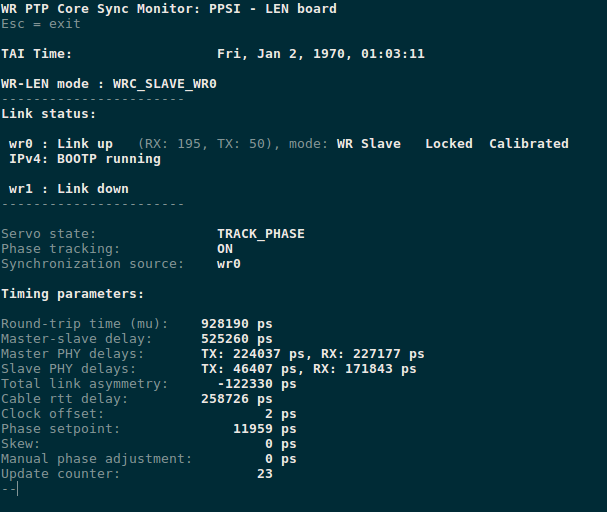
\includegraphics[width=0.7\linewidth]{imagenes/len_gui}
	\caption[Captura del monitor WR en el dispositivo WR-LEN]{Esta captura 
	muestra la información que aporta el monitor interactivo WR para el caso de 
	un nodo. Los datos más importantes son los relativos a la hora del sistema, 
	el modo de operación y el estado del servo. Además se ofrecen estadísticas 
	del enlace como el \textit{round-trip time} o la asimetría.}
	\label{fig:lengui}
\end{figure}


De las alternativas disponibles en el universo de los dispositivos WR, se ha 
utilizado la arquitectura basada en nodo, y en concreto 
WR-LENs para realizar este tipo de pruebas: por un lado, los resultados 
obtenidos se pueden extrapolar a otros diseños como el del \gls{wrs}. Esto se 
debe a que el mecanismo de sincronización es prácticamente el mismo en ambas 
arquitecturas. Y por el otro, está el sentido práctico: realizar una cadena de 
muchos equipos es complejo en cuanto a la gran necesidad de material y recursos 
en el laboratorio. El uso de equipos simples como el WR-LEN ha hecho posible 
llegar a conectar un elevado número de nodos en cascada (hasta 18) permitiendo 
así observar el comportamiento de la tecnología en una red con un gran número 
de saltos (o \textit{hops}).

El primer experimento está pensado para comprobar si efectivamente la 
sincronización se deteriora hasta el punto de no lograr sincronizar un equipo 
(aunque sea fuera del nanosegundo de diferencia).
Para ello se desplegó una red de WR-LEN conectadas en cadena, tal como muestra 
la Figura \ref{fig:chainschema}. Para comprobar la exactitud de la 
sincronización en los puntos elegidos, se toma el reloj de salida del nodo 
maestro como referencia y el reloj del nodo esclavo i-ésimo, y con la ayuda de 
un osciloscopio de alta resolución se toman muestras de la diferencia en el 
dominio del tiempo entre los flancos de subida de las señales de reloj o de los 
PPSs.

Antes de efectuar las pruebas es necesario realizar una calibración de los 
retardos de propagación típicos de los dispositivos WR-LEN necesarios por el 
modelo de enlace para el cálculo del desfase. También hace falta calcular el 
coeficiente de asimetría relacionado con la diferencia de velocidad de 
propagación entre la señal empleada para transmitir y la de recibir. El 
procedimiento para dicho proceso de calibración se encuentra descrito en 
\cite{man:calib}. Los valores obtenidos pueden reutilizarse entre dispositivos 
que mantengan la misma versión de \textit{firmware}. Reutilizar dichos valores 
conlleva una pequeña pérdida de exactitud dado que no se tienen en cuenta las 
pequeñas variaciones que existen entre tarjetas, cosa que puede parecer 
insignificante pero que toma relevancia cuando hablamos de cotas de 
sincronización que alcanzan las decenas de picosegundos de exactitud. Sin 
embargo no se ha considerado necesario llegar hasta estos extremos ya que el 
resultado principal que se pretende obtener son los valores relativos a la 
precisión, es decir, como de estable son las señales producidas por los 
dispositivos. Así pues se observarán pequeños desplazamientos en las medidas de 
desfase entre las señales de maestro y esclavo, que se irán acrecentando con 
forme se aumente el número de nodos en cascada.

Para comprobar si un nodo logra sincronizarse, además de observar las señales 
de salida, se debe consultar el monitor de estado de \textit{wr}. En la Figura 
\ref{fig:lengui} se incluye una captura de dicho monitor. Como se ha 
mencionando anteriormente, este primero experimento busca 
determinar en que momento un nodo es incapaz de sincronizarse con el resto de 
la red. Para determinarlo, se debe ir conectando uno a uno cada dispositivo y 
comprobar el estado de la sincronización es \textit{Track-Phase}. 
Además se puede ir comprobando que la diferencia en tiempo entre las señales de 
\gls{pps} del maestro \textit{free-running} y de cada nodo sea inferior al 
nanosegundo. Las pruebas se han tomado por período de una hora y cada 
experimento se ha repetido tres veces para comprobar la consistencia de los 
resultados.

\begin{figure}
	\centering
	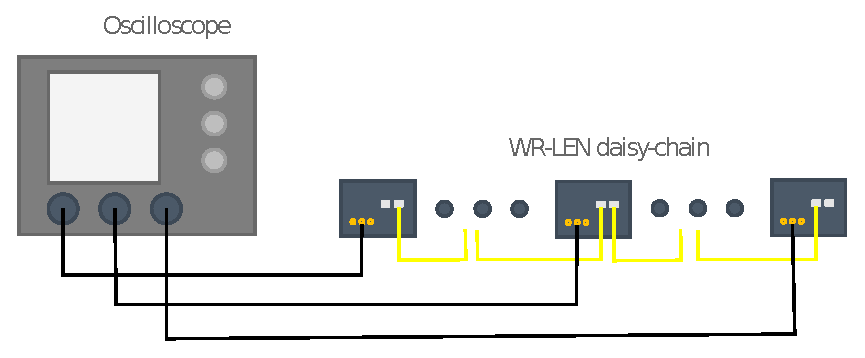
\includegraphics[width=0.7\linewidth]{imagenes/chain_schema}
	\caption[Esquema de conexión para los experimentos de escalabilidad.]{El 
	esquema muestra como se han conectado los diferentes nodos que han 
	compuesto la red WR para los experimentos de escalabilidad. Cada nodo actúa 
	como esclavo del nivel inferior y como maestro del siguiente (cascada).}
	\label{fig:chainschema}
\end{figure}

\begin{table}
	% increase table row spacing, adjust to taste
	\renewcommand{\arraystretch}{1.3}
	% if using array.sty, it might be a good idea to tweak the value of
	% \extrarowheight as needed to properly center the text within the cells
	\caption{Medidas de desfase para el primer experimento de la cascada de 
	WR-LEN con 18 nodos.}
	\label{tab:cascada1}
	\centering
	% Some packages, such as MDW tools, offer better commands for making tables
	% than the plain LaTeX2e tabular which is used here.
	\begin{tabular}{|c||c||c||c|}
		\hline
		Desfase & Mean & $\sigma$ & peak-to-peak \\
		\hline
		Maestro al 10º nodo & -212.51 ps & 45.653 ps & 312.50 ps \\
		\hline
		Maestro al 15º nodo & -500.66 ps & 174.50 ps & 1.0731 ns \\
		\hline
		Maestro al 18º nodo & -573.45 ps & 490.17 ps & 2.6487 ns \\
		\hline
	\end{tabular}
\end{table}

En el contexto de este análisis los valores más relevantes extraídos son los 
correspondientes a la desviación típica y al llamado \textit{peak-to-peak} que 
no es más que la diferencia entre el valor máximo y el mínimo. Con el primero 
nos podemos hacer una idea del ruido presente en el sistema y con el segundo se 
comprueba cuando, en el peor de los casos, la sincronización pierde en algún 
momento el nanosegundo de exactitud. ¿Por qué no interesa el valor medio? Al 
principio de la sección se ha mencionado que se han utilizado los mismos 
parámetros de calibración para todos los nodos. Esto es algo típico y que 
funciona bastante bien cuando nos encontramos dentro de un escenario usual de 
red. Sin embargo, es totalmente posible realizar una calibración por nodo 
consiguiendo así que el valor medio esté centrado en 0. Dado que el foco de 
este análisis es el ruido y sus consecuencias, no se ha considerado relevante 
invertir tiempo en realizar un proceso de calibración completo que habría 
supuesto invertir mucho tiempo.

Los resultados numéricos de este primer experimento se incluyen en la Tabla 
\ref{tab:cascada1} y también se puede observar la distribución que siguen las 
muestras tomadas en la Figura \ref{fig:histexp1}. Se incluyen únicamente los 
resultados en los nodos 10º, 15º y 18º por motivos de reproducibilidad del 
experimento. Dado que el osciloscopio cuenta con 4 canales de entrada y uno de 
ellos es el utilizado por la referencia, solo se pueden tomar al mismo tiempo 
medidas de 3 nodos.
Del montaje inicial de la red se determinó que la sincronización 
sub-nanosegundo se consigue hasta el nodo 12º. Aunque los siguientes nodos se 
encuentran \textit{en media} dentro de rango, el análisis del peor de los casos 
muestra que es a partir del nodo 12º cuando no se puede asegurar que la 
diferencia entre la marca temporal del maestro y la del nodo sea siempre menor 
del ns \textit{explicar como se calcula eso que no es trivial}. Aún así los 
valores medios pueden ser interesantes para aplicaciones 
que no sean críticas y permitan cierta tolerancia a este fenómeno.
El otro resultado importante al que se llegó fue que a partir del nodo 18º no 
se consigue pasar de la fase de sintonización por lo que \gls{wr} no puede 
funcionar. Es decir, se comprobó que la hipótesis era cierta y el incremento 
del nivel de ruido por salto ocasiona un deterioro constante de la distribución 
de tiempo que llega hasta el punto de ser imposible sincronizar sin realizar 
ajustes en el algoritmo de control para relajar las condiciones del bucle de 
control.

Tras observar ambos resultados, se realizó una toma de medidas de desfase entre 
nodos clave: 10º, 15º y 18º. Los primeros nodos mostraban valores bajos de 
ruido por lo que resultaba más interesante analizar que pasaba cerca del punto 
donde se pierde la sincronización y al final de la cadena, donde el ruido 
comienza a ser muy elevado. Los resultados mostrados en la Tabla 
\ref{tab:cascada1} ayudan a comprender que falla para que a partir del nodo 18º 
no se consiga sintonizar. El problema se debe a el alto nivel de ruido en la 
señal que se recupera del enlace y que por tanto se sale de los límites que 
permite el bucle de control encargado de medir el desfase y disciplinar el 
reloj local. Para solucionar este problema se puede aumentar el ancho de banda 
de dicho bucle para permitir cambios más grande en frecuencia de la señal 
recuperada. Esto tiene una repercusión y es que se aumenta el nivel de ruido 
del sistema debido a que el filtro formado por el bucle de control reacciona a 
un mayor ancho de banda siendo vulnerable a perturbaciones no deseadas en la 
señal de reloj. 



Otro de las pruebas realizadas busca comprobar una de las hipótesis del procolo 
WR de que la longitud 
del enlace de fibra óptica no tiene un efecto considerable sobra la precisión 
de la sincronización (siempre considerando una longitud dentro del rango de 
operación de los \gls{sfp}s utilizados). Para ello se replicó el montaje en 
cadena, pero utilizando menos nodos (15) pues los valores de los nodos finales 
en cadenas largas son muy inestables y aportan poca confianza estadística a la 
hora de determinar si hay diferencia o no entre usar un enlace corto o no. Las 
medidas de desfase se han tomado en los nodos 13º, 14º y 15º, usando un enlace 
de 5 km entre los nodos 13º y 14º.

\begin{table}
	% increase table row spacing, adjust to taste
	\renewcommand{\arraystretch}{1.3}
	% if using array.sty, it might be a good idea to tweak the value of
	% \extrarowheight as needed to properly center the text within the cells
	\caption{Medidas de desfase para el segundo experimento de la cascada de 
		WR-LEN usando fibras cortas.}
	\label{tab:cascada2}
	\centering
	\begin{tabular}{|c||c||c||c|}
		\hline
		Desfase & Mean & $\sigma$ & peak-to-peak \\
		\hline
		Maestro al 13º nodo & -368.82 ps & 117.08 ps & 694.23 ps \\
		\hline
		Maestro al 14º nodo & -367.75 ps & 173.45 ps & 971.43 ps \\
		\hline
		Maestro al 15º nodo & -766.19 ps & 235.77 ps & 1.373 ns \\
		\hline
	\end{tabular}
\end{table}

\begin{table}
	% increase table row spacing, adjust to taste
	\renewcommand{\arraystretch}{1.3}
	% if using array.sty, it might be a good idea to tweak the value of
	% \extrarowheight as needed to properly center the text within the cells
	\caption{Medidas de desfase para el segundo experimento de la cascada de 
		WR-LEN usando un enlace de 5 km entre los nodos 13º y 14º.}
	\label{tab:cascada3}
	\centering
	% Some packages, such as MDW tools, offer better commands for making tables
	% than the plain LaTeX2e tabular which is used here.
	\begin{tabular}{|c||c||c||c|}
		\hline
		Desfase & Mean & $\sigma$ & peak-to-peak \\
		\hline
		Maestro al 13º nodo & -341.08 ps & 101.02 ps & 507.05 ps \\
		\hline
		Maestro al 14º nodo & -271.06 ps & 234.52 ps & 859.52 ps \\
		\hline
		Maestro al 15º nodo & -700.65 ps & 203.93 ps & 1.5425 ns \\
		\hline
	\end{tabular}
\end{table}

Los resultados se incluyen en la Tabla \ref{tab:cascada2} para el caso de todos 
los enlaces con fibras cortas, y en la Tabla \ref{tab:cascada3} para el del 
enlace de varios kilómetros. Al igual que para el primer experimento se 
incluyen los histogramas de la distribución de las muestras en las Figuras 
\ref{fig:histexp2} y \ref{fig:histexp3} respectivamente. La diferencia 
observada entre los dos experimentos muestra que no hay diferencia 
significativa (los valores tienen una gran dispersión) entre el uso de un 
enlace de varios kilómetros o uno casi despreciable, tanto en el caso del nodo 
conectado con el enlace como en el siguiente. Además los resultados son 
consistentes con lo visto en el primero experimento: el nodo 13º se encuentra 
fuera (por poco) del ns en el peor de los casos, y el nodo 15º presenta una 
dispersión en torno a los 200 ps.

\begin{figure}
	\centering
	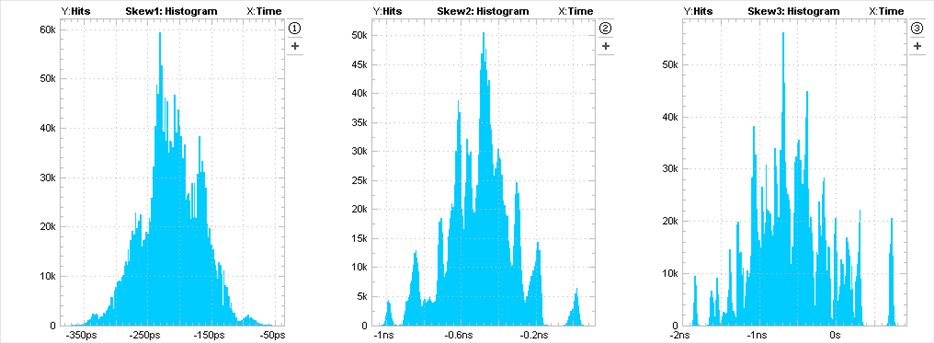
\includegraphics[width=0.7\linewidth]{imagenes/hist_exp1}
	\caption[Histograma para cadena de 18 WR-LEN]{Los histogramas muestran la 
	distribución de las muestras correspondientes a la diferencia entre las 
	señales de PPS en el maestro y la de los nodos 10, 15 y 18.}
	\label{fig:histexp1}
\end{figure}

\begin{figure}
	\centering
	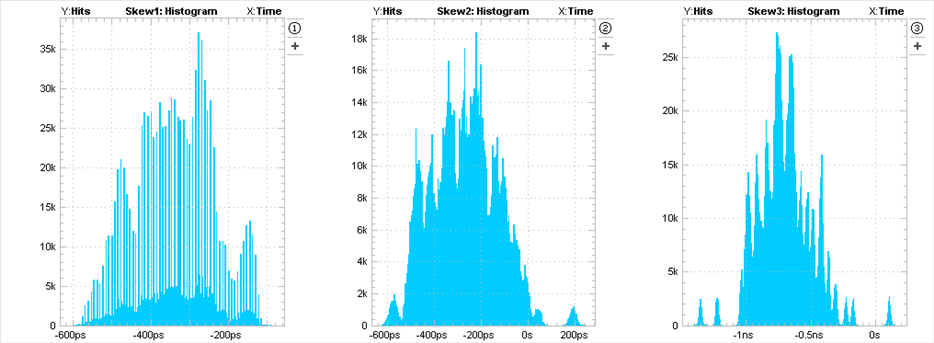
\includegraphics[width=0.7\linewidth]{imagenes/hist_exp3}
	\caption[Histograma para cadena de 15 WR-LEN]{Los histogramas muestran la 
		distribución de las muestras correspondientes a la diferencia entre las 
		señales de PPS en el maestro y la de los nodos 10, 15 y 18.}
	\label{fig:histexp2}
\end{figure}

\begin{figure}
	\centering
	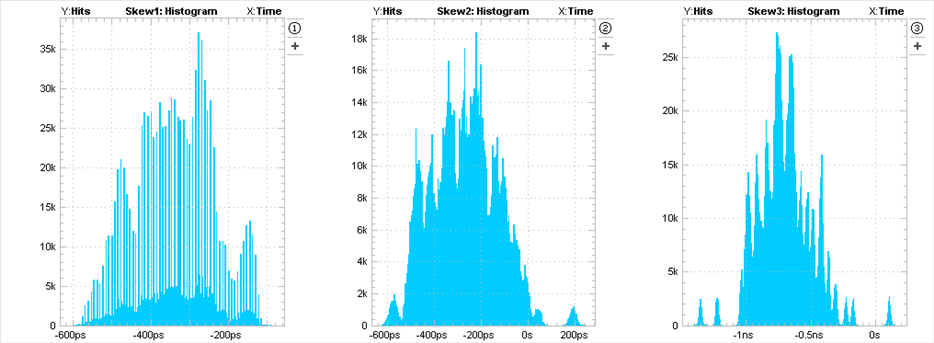
\includegraphics[width=0.7\linewidth]{imagenes/hist_exp3}
	\caption[Histograma para cadena de 15 WR-LEN con un enlace de 5km]{Los 
	histogramas muestran la distribución de las muestras correspondientes a la 
	diferencia entre las señales de PPS en el maestro y la de los nodos 10, 15 
	y 18.}
	\label{fig:histexp3}
\end{figure}

\subsubsection{Conclusiones}

Los experimentos realizados sobre una red de dispositivos \gls{wr} conectados 
en cascada han arrojado varios resultados interesantes y han permitido 
comprobar las hipótesis acerca del efecto del ruido en el sistema y us 
consecuencias:

\begin{itemize}
	\item Se ha realizado una caracterización de la implementación \gls{wrc2p}, 
	la cual extiende la funcionalidad de la arquitectura clásica de nodo 
	\gls{wr} manteniendo un diseño alojable en \gls{fpga}s de perfil bajo. Dado 
	que dicha implementación es relativamente nueva, era importante comprobar 
	que el nuevo diseño cumple las especificaciones básicas del protocolo  
	\gls{wr} antes de trabajar en las posibles mejoras.
	
	\item Se han obtenido resultados muy interesantes en cuanto a los límites 
	de la tecnología, observando que no se consiguen sincronizar más de 18 
	equipos en cadena. Este tipo de pruebas no se había realizado hasta la 
	fecha con un número tan elevado de equipos \gls{wr} por lo que dichos 
	resultados son de gran utilidad para el resto de la comunidad. Si bien los 
	resultados se han obtenido usando equipos de bajo perfil, la electrónica de 
	control es en su mayor parte idéntica a la usada por el \gls{wrs} por lo 
	que se puede extrapolar las conclusiones pensando que quizás en el caso de 
	una cadena de 18 \gls{wrs}s se podría obtener cierta mejora gracias a 
	contar con una \gls{fpga} de perfil alto que cuenta con 
	\textit{transceivers} GTX en lugar 
	de GTP.
	
	\item Se ha comprobado la hipótesis de que gracias al nuevo modelo de 
	enlace presente en \gls{wr} se consigue calibrar de forma dinámica la 
	longitud del enlace de fibra óptica mediante la utilización del parámetro 
	de asimetría.
\end{itemize}

Además he podido comprobar de primera mano que aspectos son mejorables y la 
posible línea de trabajo futuro. En cuanto a la arquitectura de nodo, he 
detectado una serie de problemas que merece la pena discutir. En primer lugar, 
hay que entender ciertas decisiones del diseño inicial que se pudieron tomar 
para realizar un sistema que fuera sencillo y mantuviese los costes bajos. Con 
esto me refiero a la ausencia de un microprocesador físico externo que permita 
obtener un mayor rendimiento y flexibilidad de desarrollo para el \textit{sw} 
de la plataforma. El código \textit{sw} actual de un nodo se ejecuta en 
procesador embebido, el LM32. Este, cuenta con unos recuros muy limitados y se 
nota 
bastante a la hora de desarrollar para esta plataforma. Al incorporar una 
\gls{fpga} de perfil bajo, el número de recursos disponibles es limitado: hay 
pocas puertas lógicas disponibles y el número de bloques de memoria RAM es 
bajo. Eso provoca que el rendimiento de ejecución del LM32 sea bastante bajo y 
el desarrollo de nuevas características está limitado por la falta de recursos. 
Hay que tener en cuenta que este sistema se pensó en un primer momento para 
gestionar una única interrupción del \textit{Soft-PLL} y realizar el cálculo 
del desfase en tiempo real. Es el caso del \gls{wrs}, donde la única función 
del LM32 es esa. En el desarrollo de la arquitectura de nodo, al carecer de un 
procesador físico disponible, se tuvo que incluir en el \textit{sw} embebido 
del LM32 todos los programas de interfaz con el usuario, el demonio \gls{ptp} y 
cualquier característica que no se implementa en HDL. Con forme el diseño ha 
ido aumentando en complejidad, la sobrecarga de este procesador se ha hecho 
evidente, llegando al punto de que el actual diseño del \gls{wrc2p} incluido en 
la WR-LEN no permite incluir ninguna funcionalidad extra por falta de memoria 
RAM y de capacidad de cómputo. También cabe mencionar el poco soporte para 
depuración que presenta este tipo de sistema, llevando mucho más tiempo 
desarrollar en esta plataforma que, por ejemplo, en un ARM.

Las herramientas de gestión incluidas en la WR-LEN son muy básicas y han hecho 
bastante laborioso realizar los experimentos con tantos nodos al mismo tiempo. 
Una vez más, debida a la falta de un SO o de una plataforma más estandarizada, 
desarrollar cualquier herramienta de control ha llevado bastante tiempo y 
actualizar el sistema no es algo trivial.

Gracias a los avances recientes en los procesos de fabricación de circuitos 
integrados actualmente podemos disponer de sistemas que integran varios 
componentes en un único chip, incluyendo una FPGA y un procesador físico en un 
mismo integrado a la vez que se mantiene un coste bajo. Como la mayoría de los 
diseños WR se basan en FPGAs de Xilinx, se puede pensar en la familia Zynq-7000 
de este fabricante como mejora a la arquitectura existente de nodo. De esta 
forma se puede incluir un SO tipo Linux que se integre de forma 

Esta nueva propuesta de plataforma se propone con más detalle en el siguiente 
capítulo, hablando de la línea de desarrollo actual y de los pasos futuros.



%\chapter{Conclusión y trabajo futuro}
%\input{referencias}
%\addcontentsline{toc}{chapter}{Blibiografía}
%
%
%

%%\chapter{Conclusiones y Trabajos Futuros}
%
%\backmatter
%%\nocite{*}
\addcontentsline{toc}{chapter}{Bibliografía}
\bibliographystyle{plain}
\bibliography{bibliografia/wr_bib}


\appendix
%\input{apendices/manual_usuario/manual_usuario}
%%\input{apendices/paper/paper}
%\input{glosario/entradas_glosario}
\addcontentsline{toc}{chapter}{Lista de Acrónimos}
\printglossaries

\thispagestyle{empty}

\end{document}
